\documentclass[11pt]{article}
\usepackage[utf8]{inputenc}

\usepackage{amsmath, amsfonts, amsthm, amssymb}
% \usepackage{fourier} 

\usepackage[margin = 0.9in]{geometry}
% \usepackage{xcolor}
\usepackage{listings}
\usepackage{color} %red, green, blue, yellow, cyan, magenta, black, white
\definecolor{mygreen}{RGB}{28,172,0} % color values Red, Green, Blue
\definecolor{mylilas}{RGB}{170,55,241}
% \usepackage[framed,numbered,autolinebreaks,useliterate]{mcode}

\usepackage{graphicx}
\usepackage{subcaption}
\usepackage[colorlinks = true,
            linkcolor = blue,
            urlcolor  = blue,
            citecolor = blue,
            anchorcolor = blue]{hyperref}

\newcommand{\parder}[2]{\frac{\partial #1}{\partial #2}}
\newcommand{\ex}{\mathbb{E}}
\newcommand{\eps}{\varepsilon}
\newtheorem{proposition}{Proposition}
% \newcommand{\oil}{\mathcal{O}}

\usepackage{tikz, pgfplots}
\usetikzlibrary{arrows, automata}
\usetikzlibrary{datavisualization.formats.functions}

\title{JTIX in Wachter (2013)}

\begin{document}

% \maketitle

\section{JTIX in Wachter (2013)}

\subsection{Summary}

\begin{proposition}
    JTIX, a model free measure of jump risk, for a $\phi$-levered consumption claim in the Wachter (2013) is an affine function of the jump intensity:
    \[JTIX_{t,\tau} = 2\Psi(a_{0,\lambda}(\tau) + a_{1,\lambda}(\tau)\lambda_t)\]
    where
    \[
        \begin{aligned}
            a_{\lambda, 0}(\tau) &= \left[\overline{\lambda}\frac{\kappa}{\kappa - b\sigma_\lambda}\tau - \overline{\lambda}\frac{\kappa}{\kappa - b\sigma_\lambda^2}\left(1-e^{-(\kappa - b\sigma_\lambda^2)\tau}\right)\right] \\
            a_{\lambda,1}(\tau) &= \frac{1}{\kappa - b \sigma_\lambda^2}\left(1-e^{-(\kappa-b\sigma_\lambda^2)\tau}\right) \\
            \Psi &= \left[1 + \phi(\mu_Z - \gamma\sigma_Z^2) + \frac{1}{2}\phi^2(\sigma_Z^2 + (\mu_Z - \gamma\sigma_Z^2)^2) - e^{\phi(\mu_Z - \gamma\sigma_Z^2) + \frac{1}{2}\phi^2\sigma_Z^2}\right]e^{-\frac{1}{2}(2\mu_Z \gamma - \gamma^2\sigma_Z^2)} \\
        \end{aligned}
    \]
\end{proposition}

This proposition implies that JTIX in the Wachter (2013) model inherits a similar slow moving behavior of the disaster intensity.

\begin{proposition}
    $JTIX_{t,\tau}$ has a distribution $JTIX_{t,\tau} \sim 2\Psi (a_{\lambda, 0}(\tau) + a_{\lambda, 1}(\tau)\xi)$ where  $\xi$ has a Gamma distribution $\xi \sim \Gamma(\alpha, \beta)$ with location parameter $\alpha$ and scale parameters $1/\beta$. $\alpha$ and $\beta$ equal to
    \[\alpha = \frac{2\kappa}{\sigma_\lambda^2}\overline{\lambda}, \ \beta = \frac{2\kappa}{\sigma_\lambda^2}\]
\end{proposition}

This proposition gives a way to simulate the distribution of JTIX within a Wachter (2013) model. In Figure \ref{fig:JTIX_wachter2013}, we show the empirical distributions for daily log-JTIX based on SPX options for 30, 90 and 180 days maturities. We compare them with theoretical distributions within the Wachter (2013) model based on propositions 1 and 2

\begin{figure}[htbp!]
    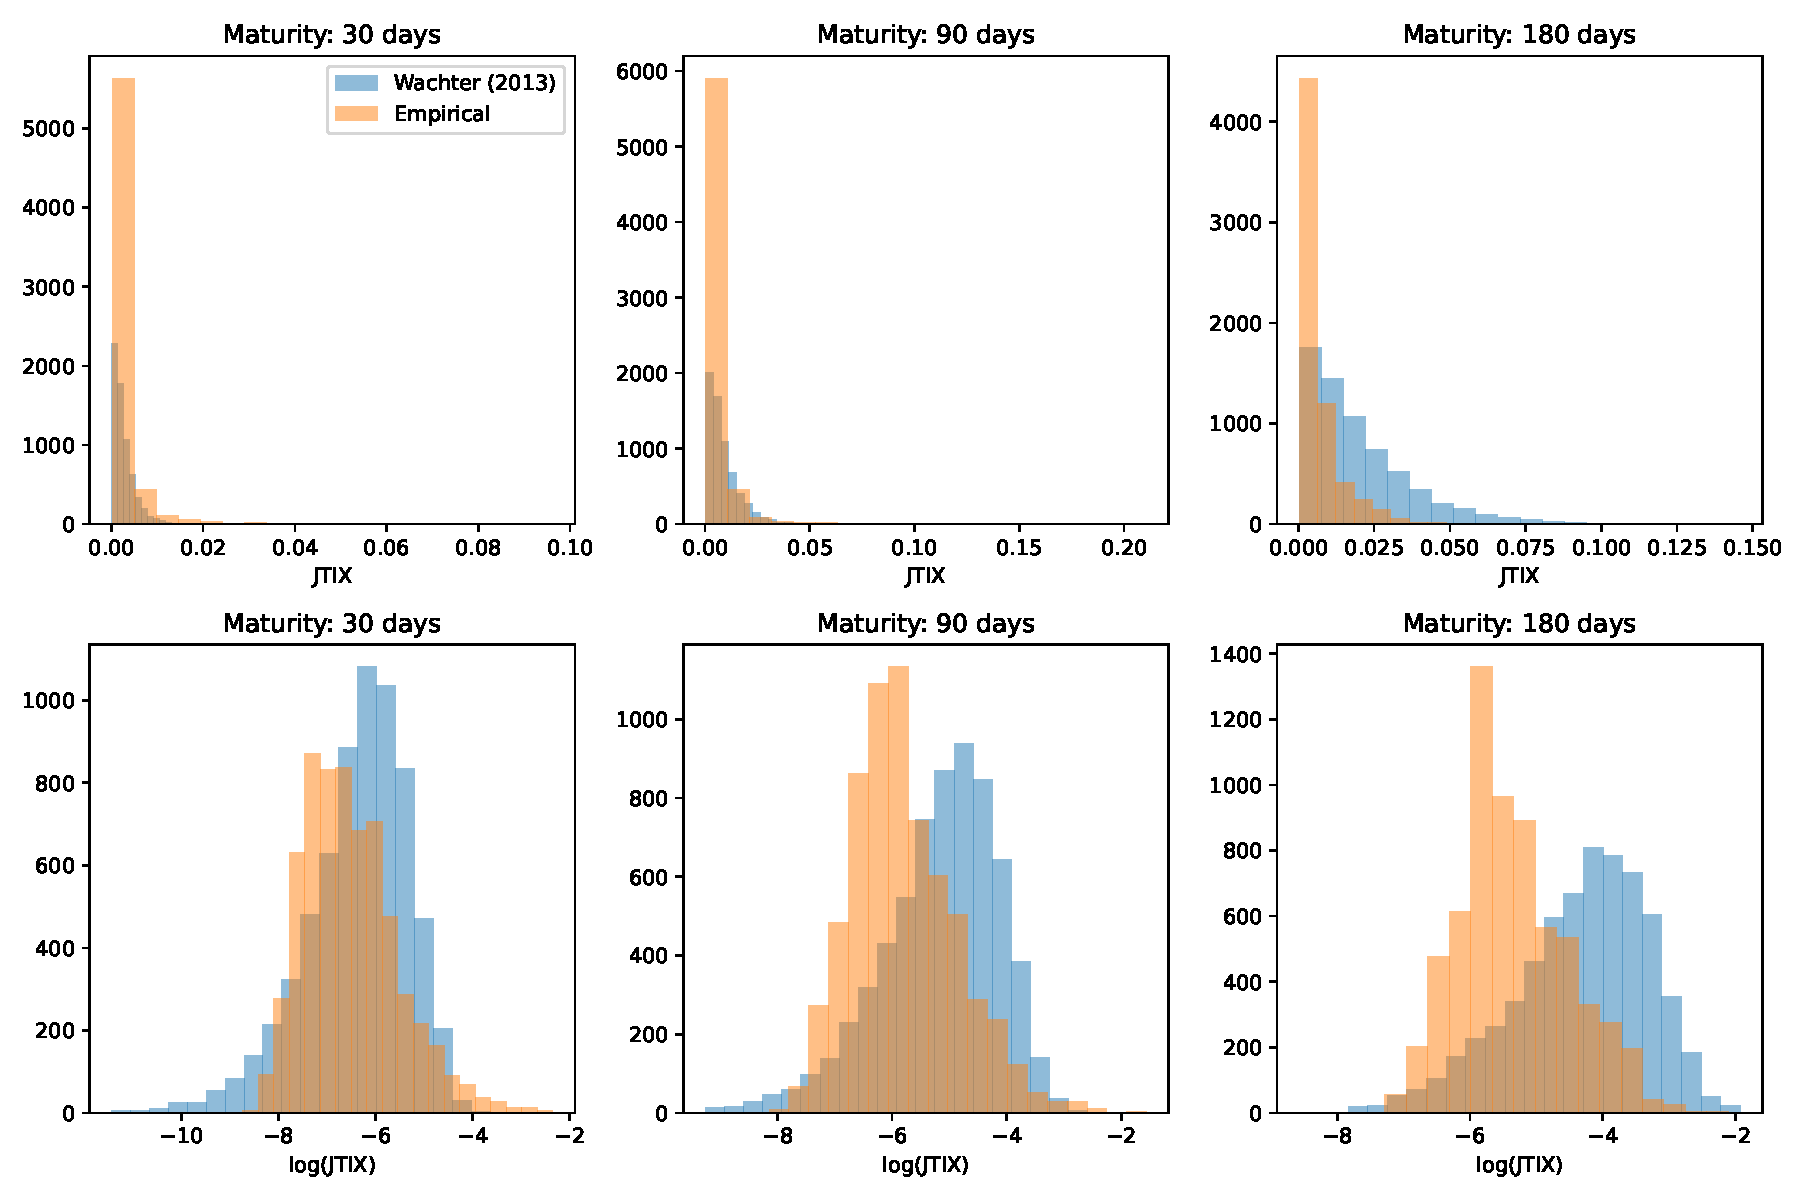
\includegraphics[width=\textwidth]{../../SS_figures/JTIX_wachter2013.pdf}
    \caption{Comparing JTIX in the data and in Wachter 2013}
    \label{fig:JTIX_wachter2013}
\end{figure}

Proposition 1 provideds us with a straighforward way to invert the JTIX measure to get the disaster intensity within the Wachter (2013). We present this inversion in Figure \ref{fig:intensity_from_JTIX} based on 30, 90 and 180 day.

\begin{figure}[htbp!]
    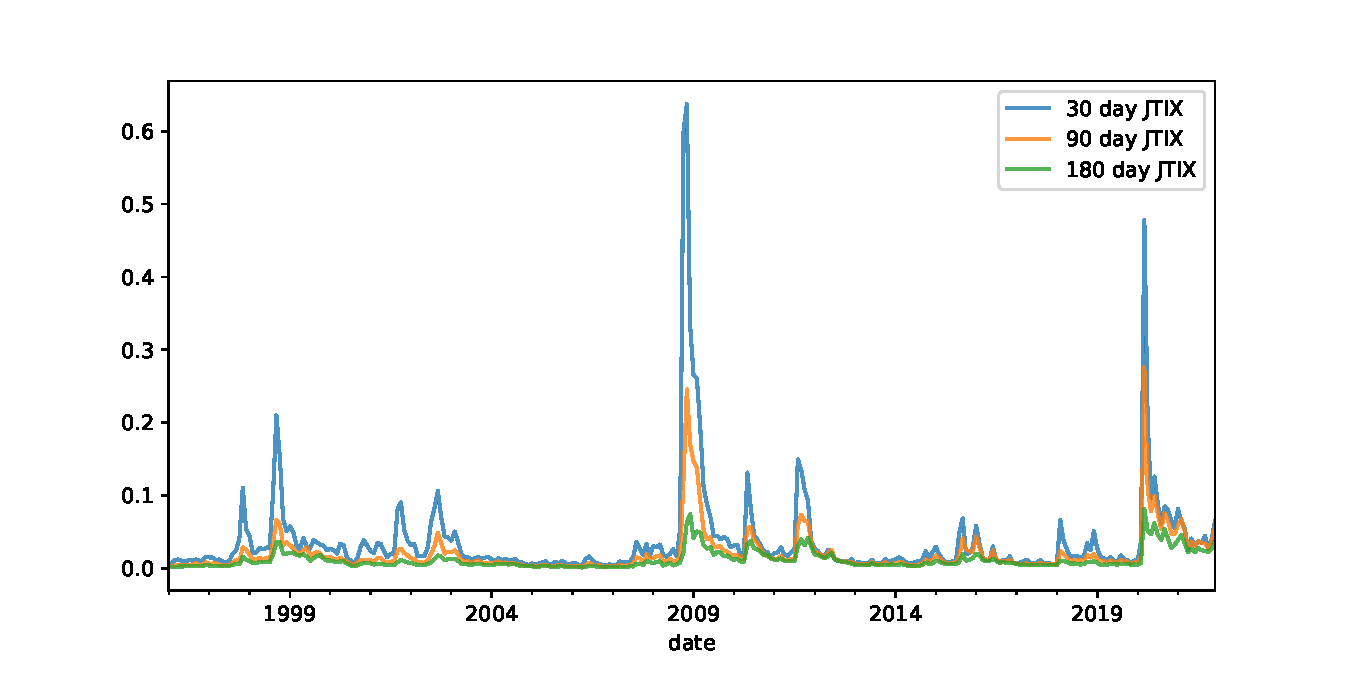
\includegraphics[width=\textwidth]{../../SS_figures/intensity_from_JTIX.pdf}
    \caption{Comparing JTIX in the data and in Wachter 2013}
    \label{fig:intensity_from_JTIX}
\end{figure}

Finally, we compare the disaster intensity obbtained bby inverting JTIX with the from inverting the CAPE ratio (following section II.C from Wachter, 2013) in Figure 

\begin{figure}[htbp!]
    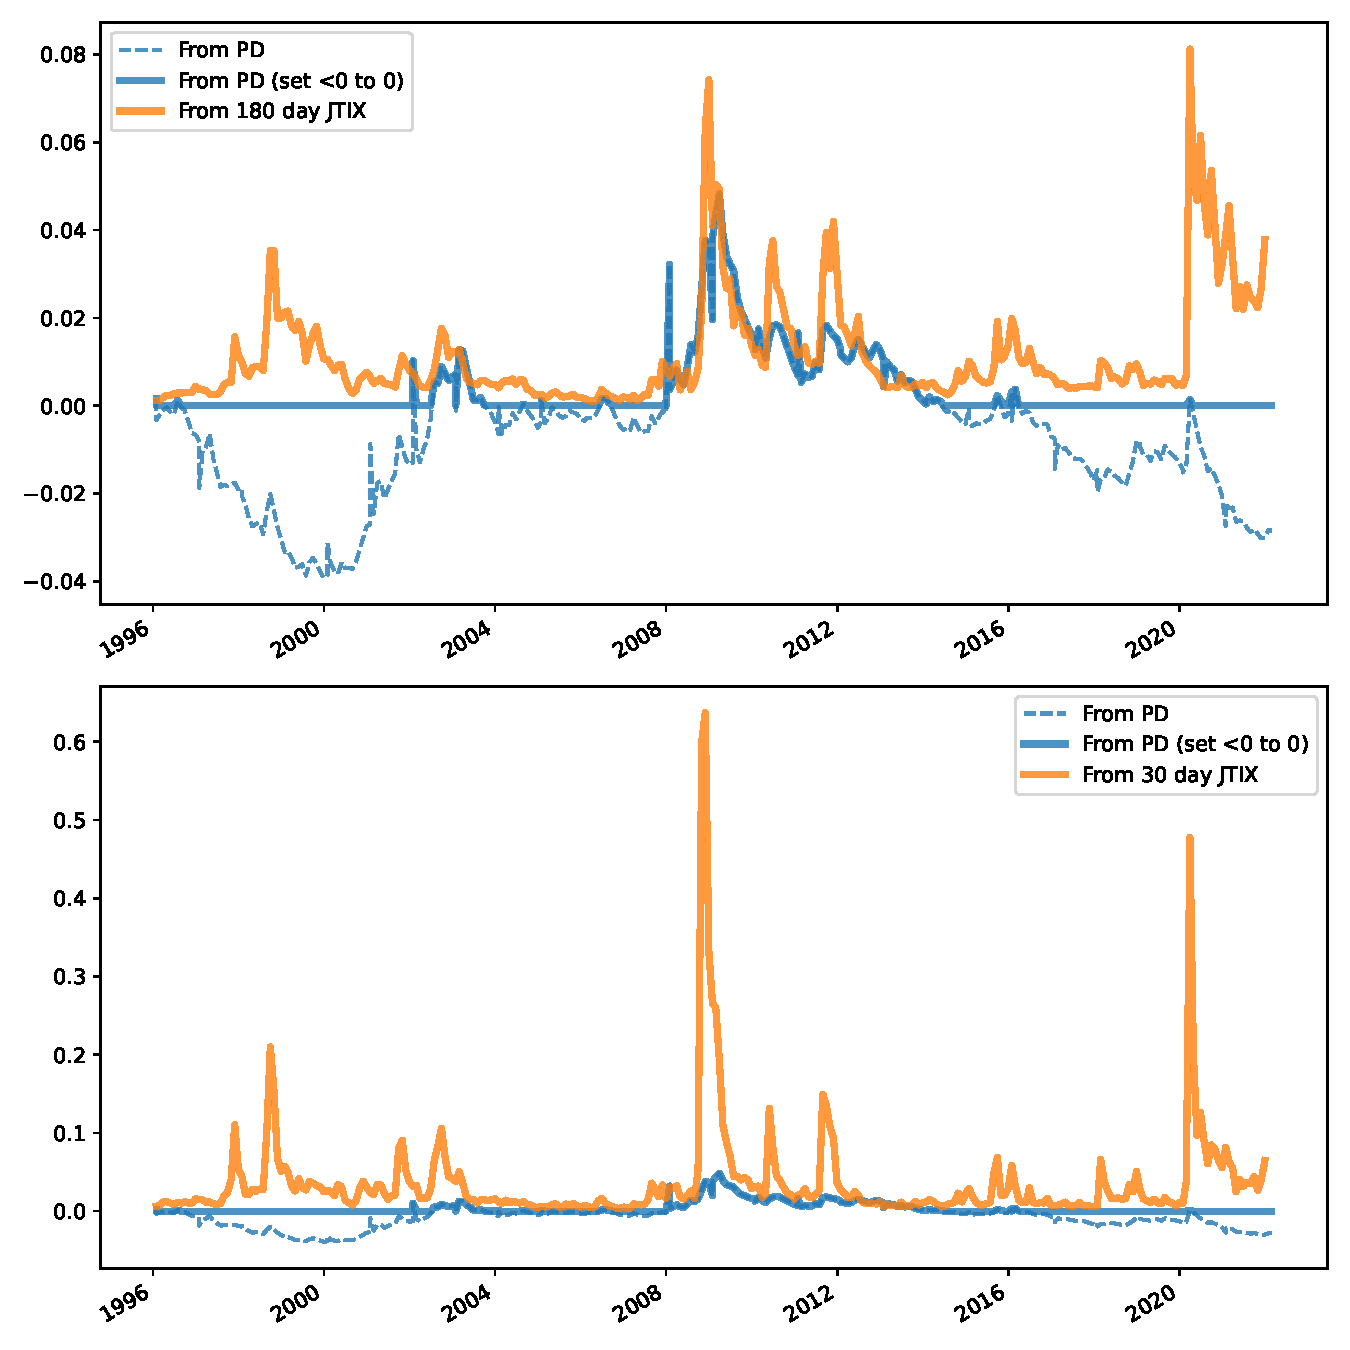
\includegraphics[width=\textwidth]{../../SS_figures/intensity_from_JTIX_vs_PD.pdf}
    \caption{Comparing JTIX in the data and in Wachter 2013}
    \label{fig:intensity_from_JTIX_vs_PD}
\end{figure}


\subsection{Overview of Wachter (2013) model}

\paragraph{Consumption Process} 

Consumption follows a jump-diffusion process
\begin{equation}\label{eq:consumption_process}
    \frac{dC_t}{C_t^{-}} = \mu_c dt + \sigma_c dB_{c,t} + (e^{Z_t} - 1)dN_t,
\end{equation}
where $dN_t$ is a Poisson counting process with time varying intensity $\lambda_t$
the process for which we describe below, the distribution of jump size
$Z_t \sim \nu(\cdot)$ is time-invariant. Rewrite the process (\ref{eq:consumption_process}) in logs
\begin{equation}\label{eq:consumption_process_logs}
    d\log C_t = \left(\mu_c - \frac{1}{2}\sigma_c^2\right)dt + \sigma_c dB_{c,t} + Z_t dN_t.    
\end{equation}
Time varying intensity follows
\begin{equation}\label{eq:intensity_process}
    d\lambda_t = \kappa (\overline{\lambda} - \lambda_t)dt + \sigma_\lambda \sqrt{\lambda_t}dB_{\lambda, t}
\end{equation}
where the square root ensures that $\lambda_t > 0$.

\paragraph{Preferences}

Wachter (2013) assumes recursive utility with EIS = 1 that allows for a semi closed form solution for the price dividend ratio. In particular, a representative agent is assumed to have a Duffie-Epstein recursive utility
\[V_t = \int_{t}^\infty f(C_s, V_s)ds\]
where
\[f(C, V) = \beta(1-\gamma)V\left(\log C - \frac{1}{1-\gamma}\log((1-\gamma)V)\right).\]

The state prices under EZ are
\begin{equation}\label{eq:state_prices_general}
    \pi_t = \exp\left\{\int_0^t f_V(C_s, V_s)ds\right\}f_C(C_t, V_t),
\end{equation}
and Wachter (2013) shows that it is equal to
\begin{equation}\label{eq:state_prices}
    \pi_t = \exp\left\{-\int_0^t (\beta b \lambda_s - \eta)ds\right\}\beta^\gamma C_t^{-\gamma}e^{a + b\lambda_t}
\end{equation}
where $b$ is defined in (\ref{eq:coefficients_zeta_b}) and
\begin{equation}\label{eq:coefficients_a_eta}
    \begin{aligned}
        a &= \frac{1-\gamma}{\beta}\left(\mu_c - \frac{1}{2}\gamma\sigma_c^2\right) + (1-\gamma)\log\beta + b \frac{\kappa \overline{\lambda}}{\beta} \\
        \eta &= \beta(1-\gamma)\log\beta - \beta a - \beta \\
    \end{aligned}
\end{equation}
Note that in equation (\ref{eq:state_prices}) the two sources of risk are (1) shocks to consumption as exemplified by $C_t^{-\gamma}$ and (2) shocks to disaster intensity as exemplified by $e^{a + b\lambda_t}$.

\paragraph{Risky assets}

An asset that is a claim to levered consumption pays a dividend
\[D_t dt = C_t^\phi dt\]
during interval $[t,t+dt]$. The price dividend for such asset is defined as
\[\frac{P_t}{D_t} = E_t\left[\int_t^\infty \frac{\pi_s}{\pi_t}\frac{D_s}{D_t}\right]\]

Wachter (2013) shows that the price dividend ratio in this model is a function of $\lambda_t$
only and can be written as
\[G(\lambda_t) \equiv \frac{P_t}{D_t} = \int_t^\infty \exp\{a_\phi(\tau) + b_\phi(\tau)\lambda_t\}d\tau\]
where
\begin{equation}\label{eq:pd_coefficients}
    \begin{aligned}
        a_\phi(\tau) &= \left((\phi-1)\left(\mu_c + \frac12(\phi-\gamma)\sigma_c^2\right) - \beta - \frac{\kappa\overline{\lambda}}{\sigma_\lambda^2}(\zeta_\phi + b \sigma_\lambda^2 - \kappa)\right)\tau 
        - \frac{2\kappa \overline{\lambda}}{\sigma_\lambda^2}\log\left(\frac{(\zeta_\phi+b\sigma_\lambda^2 - \kappa)(e^{-\zeta_\phi \tau} - 1) + 2\zeta_\phi}{2\zeta_\phi}\right) \\
        b_\phi(\tau) &= \frac{2\mathbb{E}_\nu\left[e^{(1-\gamma)Z}-e^{(\phi-\gamma)Z}\right](1-e^{-\zeta_\phi \tau})}{(\zeta_\phi + b \sigma_\lambda^2-\kappa)(1-e^{-\zeta_\phi \tau}) - 2\zeta_\phi} \\
    \end{aligned}    
\end{equation}
and constants $b$ and $\zeta_\phi$ are
\begin{equation}\label{eq:coefficients_zeta_b}
    \begin{aligned}
        \zeta_\phi &= \sqrt{(b\sigma_\lambda^2 - \kappa)^2 + 2\mathbb{E}_\nu\left[e^{(1-\gamma)Z} - e^{(\phi-\gamma)Z}\right]\sigma_\lambda^2} \\
        b          &= \frac{\kappa + \beta}{\sigma_\lambda^2} - \sqrt{\left(\frac{\kappa+\beta}{\sigma_\lambda^2}\right)^2 - 2\frac{\mathbb{E}\left[e^{(1-\gamma)Z}\right] - 1}{\sigma_\lambda^2}}  \\
    \end{aligned}  
\end{equation}

\paragraph{Linearization}

In order to solve for option prices and, in particular, map the set-up of the model
into the affine structure of Duffie, Pan and Singleton (2000), Seo and Wachter (2019)
linearize the log price dividend ratio around some $\lambda^*$ as
\[\log(\hat{G}(\lambda)) = \log(G(\lambda^*)) + \frac{G'(\lambda^*)}{G(\lambda^*)}(\lambda - \lambda^*)\]
\[\hat{G}(\lambda) = G(\lambda^*)\exp\left\{\frac{G'(\lambda^*)}{G(\lambda^*)}(\lambda - \lambda^*)\right\}\]
Denote 
\[b_\phi^* \equiv \frac{G'(\lambda^*)}{G(\lambda^*)} = \frac{1}{G(\lambda^*)}\int_0^\infty b_\phi(\tau)\exp\{a_\phi(\tau) + b_\phi(\tau)\lambda^*\}d\tau\]
so that
\begin{equation}\label{eq:linearized_pd}
    \hat{G}(\lambda) = G(\lambda^*)\exp\{b_\phi^* (\lambda - \lambda^*)\}.
\end{equation}

\subsection{Calculating JTIX in Wachter (2013)}

A model independent measure jump measure $JTIX_{t,\tau}$ equals to
\[JTIX_{t,\tau} = 2 E^Q_\nu\left[1 + \Delta Z + \frac12 (\Delta Z)^2 - e^{\Delta Z}\right]E^Q\int_t^{t+\tau} \lambda_{t+s}ds\]
where $E^Q_\nu[\cdot]$ is an expectation with respect to the distribution of the jump $\Delta Z$ of a levered consumption claim. The value of a levered consumption claim $S_t$ in Wachter (2013) model is $S_t = G(\lambda_t)C_t^\phi$ implying that conditional on a jump in consumption the jump in $\log(S_t)$ equals to $\phi \Delta Z_t$ where $\Delta Z_t$ is the size of the jump in log consumption $\log(C_t)$.
To calculate this expression within Wachter (2013) model, we split it into two parts. 

\paragraph{Jump distribution} The first part can be calculated as
\[
    \begin{aligned}
        &E^Q_\nu\left[1 + \phi Z + \frac12 (\phi Z)^2 - e^{\phi Z}\right] \\
        &= E_\nu\left[\frac{\pi_t}{\pi_{t-}}\left(1 + \phi Z + \frac12 (\phi Z)^2 - e^{\phi Z}\right)\right] \\
        &= E_\nu\left[\frac{\exp\left\{-\int_0^t (\beta b \lambda_s - \eta)ds\right\}\beta^\gamma C_{t}^{-\gamma}e^{a + b\lambda_t}}{\exp\left\{-\int_0^{t-} (\beta b \lambda_s - \eta)ds\right\}\beta^\gamma C_{t-}^{-\gamma}e^{a + b\lambda_{t-}}}\left(1 + \phi Z + \frac12 (\phi Z)^2 - e^{\phi Z}\right)\right] \\
        &= E_\nu\left[\frac{C_{t}^{-\gamma}}{C_{t-}^{-\gamma}}\left(1 + \phi Z + \frac12 (\phi Z)^2 - e^{\phi Z}\right)\right] \\
        &= E_\nu\left[\left(e^{Z}\right)^{-\gamma}\left(1 + \phi Z + \frac12 (\phi Z)^2 - e^{\phi Z}\right)\right] \\
    \end{aligned}
\]
This expression can be evaluated under the assumption that $Z \sim \mathcal{N}(\mu_z,\sigma_Z)$ as follows
\[
    \begin{aligned}
        &E^Q_\nu\left[1 + \phi Z + \frac12 (\phi Z)^2 - e^{\phi Z}\right] \\
        &= E_{\tilde{\nu}}\left[\left(1 + \phi Z + \frac12 (\phi Z)^2 - e^{\phi Z}\right)\right]e^{-\frac{1}{2}(2\mu_Z \gamma - \gamma^2\sigma_Z^2)} \\
    \end{aligned}
\]
where, under $\tilde{\nu}$, $Z\sim\mathcal{N}(\mu_Z - \gamma\sigma_Z^2,\sigma_Z)$ which can be shown by explicitly writing normal density and collecting $Z$ variables. Therefore
\[
    \Psi = \left[1 + \phi(\mu_Z - \gamma\sigma_Z^2) + \frac{1}{2}\phi^2(\sigma_Z^2 + (\mu_Z - \gamma\sigma_Z^2)^2) - e^{\phi(\mu_Z - \gamma\sigma_Z^2) + \frac{1}{2}\phi^2\sigma_Z^2}\right]e^{-\frac{1}{2}(2\mu_Z \gamma - \gamma^2\sigma_Z^2)}
\]

\paragraph{Intensity}

Following Proposition 6F in Duffie (2004), the risk neutral expectation is
\begin{equation}\label{eq:risk_neutral_exp_definition}
    E^Q\left[\lambda_{t+s}\right] = E\left[\exp\left\{\int_t^{t+s} r_s ds\right\}\frac{\pi_{t+s}}{\pi_t}\lambda_{t+s}\right]
\end{equation}
where $r_s$ is the short rate process
\[r_s = \beta + \mu - \gamma\sigma^2 + \lambda_tE_\nu\left[e^{-\gamma Z}(e^Z - 1)\right].\]

\paragraph{Transform method} 

To calculate expectation in (\ref{eq:risk_neutral_exp_definition}), we can utilize the transform method from Duffie, Pan and SIngleton (2000). To do this, first, define the state variable
\[
    X_t = \begin{pmatrix}
        \log C_t - \log C_0 \\ \lambda_t
    \end{pmatrix},
\]
with law of motion
\[
    dX_t = \mu(X_t) dt +  \sigma(X_t)\begin{pmatrix}
        dB_t \\ dB_{\lambda,t}
    \end{pmatrix} + \begin{pmatrix}
        Z_t \\ 0
    \end{pmatrix}dN_t.
\]
Next define $(K_0, K_1, H_0, H_1, l_0, l_1, \rho_0, \rho_1)$, parameters $(u, v)$ and function $\theta(c)$:
\begin{itemize}
    \item Drift of $X_s$: 
    \[\mu(X_t) = K_0 + K_1 X_t = \begin{pmatrix} \mu -\frac{1}{2}\sigma_c^2 \\ \kappa \overline{\lambda} \end{pmatrix} + \begin{pmatrix} 0 & 0 \\ 0 & -\kappa\end{pmatrix}\begin{pmatrix} \log C_s/C_0 \\ \lambda_s\end{pmatrix}\]
    \item Element $(i,j)$ of the covariance matrix of $X_t$:
    \[\sigma(X_s) = \begin{pmatrix} \sigma_c & 0 \\ 0 & \sigma_\lambda \sqrt{\lambda_s} \end{pmatrix} \Rightarrow \sigma(X_s)\sigma(X_s)^T = \begin{pmatrix} \sigma_c^2 & 0 \\ 0 & \sigma_\lambda^2\lambda_s\end{pmatrix}\]
    implying
    \[(\sigma(X_t)\sigma(X_t)^T)_{11} = (H_0)_{11} + (H_1)_{11}X_s = \sigma_c^2 + (0, \ 0)\cdot X_s\]
    \[(\sigma(X_t)\sigma(X_t)^T)_{12} = (H_0)_{12} + (H_1)_{12}X_s = 0 + (0, \ 0)\cdot X_s\]
    \[(\sigma(X_t)\sigma(X_t)^T)_{21} = (H_0)_{21} + (H_1)_{21}X_s = 0 + (0, \ 0)\cdot X_s\]
    \[(\sigma(X_t)\sigma(X_t)^T)_{22} = (H_0)_{22} + (H_1)_{22}X_s = 0 + (0, \ \sigma_\lambda^2)\cdot X_s\]
    \item Jump intensity $\lambda(X_s)$
    \[\lambda(X_s) = l_0 + l_1 \cdot X_s = 0 + (0, \ 1)X_s\]
    \item "Discount rate" $R(X_s)$: 
    \[R(X_s) = \rho_0 + \rho_1 \cdot X_s = -(\mu - \gamma\sigma^2 + \beta(1-\gamma)\log(\beta) - \beta a) + (0, \ b \beta - E\left[e^{-\gamma Z}(e^Z-1)\right])X_s\]
    \item Variable multiplying the state in the exponent $u = (-\gamma, b)$
    \item Variable multiplying the state $v = (0, 1)$
    \item Function capturing the properties of the jump size
    \[\theta(c) = \int_{R^2} e^{c_1 Z_1 + c_2 Z_2} d\nu(Z) = E_\nu[e^{c_1 Z_t}].\]
\end{itemize}
Under these definitions, the expectation in (\ref{eq:risk_neutral_exp_definition}) can be written as
\begin{equation}\label{eq:risk_neutral_exp_transform}
    E^Q\left[\lambda_{t+\tau}\right]
    =E\left[\exp\left\{\int_t^{t+\tau}(\rho_0 + \rho\cdot X_s)ds\right\}(v \cdot X_{t+\tau})e^{u\cdot X_{t+\tau}}\right] e^{-b\lambda_t}
\end{equation}

Duffie, Pan and Singleton (2000) show expectation in (\ref{eq:risk_neutral_exp_transform}) can be calculated as
\[\exp\{\alpha(t) + \beta(t)\cdot X_t\}(A(t) + B(t)\cdot X_t)\]
where functions $\alpha(t), \beta(t), A(t)$ and $B(t)$ satisfy the following differential equations
\[
    \left\{\begin{aligned}
        \dot{\beta}(t)  &= \rho_1 + K_1^T\beta(t)-\frac{1}{2}\begin{pmatrix} \sum_{ij} (\beta(t))_i (H_1)_{ij1} (\beta(t))_j \\ \sum_{ij} (\beta(t))_i (H_1)_{ij2} (\beta(t))_j \end{pmatrix} - l_1(\theta(\beta(t)) - 1) &\text{ subject to } \beta(t+\tau) = u \\
        \dot{\alpha}(t) &= \rho_0 + K_0 \cdot \beta(t)-\frac{1}{2}\beta(t)^T H_0 \beta(t) - l_0(\theta(\beta(t)) - 1) &\text{ subject to } \alpha(t+\tau) = 0\\
        \dot{B}(t) &= -K_1^T B(t) - \begin{pmatrix} \sum_{ij} (\beta(t))_i (H_1)_{ij1} (B(t))_j \\ \sum_{ij} (\beta(t))_i (H_1)_{ij2} (B(t))_j \end{pmatrix} - l_1 \nabla\theta(\beta(t))\cdot B(t) &\text{ subject to } B(t+\tau) = v\\
        \dot{A}(t) &= -K_0 \cdot B(t) - \beta(t)^T H_0 B(t) - l_0\nabla\theta(\beta(t))B(t) &\text{ subject to } A(t+\tau) = 0\\
    \end{aligned} \right.
\]
It follows from this system that $\dot{\beta}(s)_1 = 0 \ \forall \ s$. Additionally, but substituting the constants defined in Wachter (2013), it can be shown that $\dot{\beta}(t+\tau)_2 = 0$ and, therefore, $\dot{\beta}(s)_2 = 0 \ \forall \ s$. These two conditions imply that $\beta(t) = u = (-\gamma, b)$. Using this solutions for $\beta(s)$ we can also show that $\dot{\alpha}(s) = 0 \ s \forall \ s$ and, therefore, $\alpha(s) = 0 \ \forall \ s$. It is also the case that $\dot{B}(s)_1 = 0 \ s \forall \ s$. As a result, the system symplifies to
\[
    \left\{\begin{aligned}
        \dot{B}(t)_2 &= (\kappa - \sigma_\lambda^2 b)B(t)_2 & \text{ subject to } B(t+\tau)_2 = 1 \\
        \dot{A}(t) &= -\kappa \overline{\lambda} B(t)_2 &\text{ subject to } A(t+\tau) = 0\\
    \end{aligned} \right.
\]
This system can bbe solved in closed form
\[
    \left\{\begin{aligned}
        B(t)_2 &= e^{-(\kappa - \sigma_\lambda^2 b)\tau} \\
        A(t) &= \frac{\kappa}{\kappa - \sigma_\lambda^2 b}\left(1-e^{-(\kappa-\sigma_\lambda^2 b)\tau}\right)\\
    \end{aligned} \right. 
\]
Combining these solution we can write the expectation as
\[E^Q[\lambda_{t+\tau}] = e^{b\lambda_t}\left(\frac{\kappa}{\kappa - \sigma_\lambda^2 b}\left(1-e^{-(\kappa-\sigma_\lambda^2 b)\tau}\right) + e^{-(\kappa - \sigma_\lambda^2 b)\tau}\lambda_t\right)e^{-b\lambda_t}.\]
Finally, we can integrate this expression to get
\[\int_0^\tau E^Q_0[\lambda_{t+s}]ds = \underbrace{\left[\overline{\lambda}\frac{\kappa}{\kappa - b\sigma_\lambda}\tau - \overline{\lambda}\frac{\kappa}{\kappa - b\sigma_\lambda^2}\left(1-e^{-(\kappa - b\sigma_\lambda^2)\tau}\right)\right]}_{a_{\lambda, 0}(\tau)} + \underbrace{\frac{1}{\kappa - b \sigma_\lambda^2}\left(1-e^{-(\kappa-b\sigma_\lambda^2)\tau}\right)}_{a_{\lambda,1}(\tau)}\lambda_t\]

\paragraph{Limiting Distribution of JTIX}

To calculate the limiting distribution of the measure we proceed in two steps. First, we note that $\lambda_t$ has a stationary Gamma distribution $\propto \lambda^{\alpha - 1}e^{-\beta \lambda}$. This can be verified by writing the Kolmogorov Forward Equation
\[\frac{\partial p(\lambda, t)}{\partial t} = -\frac{\partial }{\partial \lambda}[\kappa(\overline{\lambda} - \lambda)p(\lambda, t)] + \frac{\partial^2}{\partial \lambda^2}\left[\frac{\sigma_\lambda^2 \lambda}{2}p(\lambda,t)\right],\]
setting $\partial p/\partial t = 0$ and substituting $p(\lambda) = c \lambda^{\alpha - 1}e^{-\beta \lambda}$. By setting the coefficients multiplying $\lambda$ and $\lambda^2$ to zero we get
\[\alpha = \frac{2\kappa}{\sigma_\lambda^2}\overline{\lambda}, \ \beta = \frac{2\kappa}{\sigma_\lambda^2}.\]
Second, we draw random variables $\lambda^{(i)}$'s from the Gamma distribution and transform then to get 
\[\log(JTIX)^{(i)} = \log(\Psi(a_{\lambda,0}(\tau) + a_{\lambda,1}(\tau)\lambda^{(i)})).\]
We then compare the distribution of JTIX in Wachter (2013) and in the data for different maturities.



\end{document}



% \subsection{Option prices}

% The price of a put with strike $K$ is
% \[P(S_0, K, T) = E_t\left[\frac{\pi_T}{\pi_0}(K - S_T)^+\right]\]
% Define a normalized put price $P_n\equiv P/S_0$ and a normalized strike $K_n \equiv K/S_0$
% \begin{equation}\label{eq:norm_option_price}
%     P_n(S_0, K_n, T) 
%     = E_t\left[\frac{\pi_T}{\pi_0}\left(K_n - \frac{S_T}{S_0}\right)^+\right]
%     = E_t\left[\frac{\pi_T}{\pi_0}K_n \mathbb{I}\left(\frac{S_T}{S_0} \le K_n\right)\right] - 
%     E_t\left[\frac{\pi_T}{\pi_0}\frac{S_T}{S_0} \mathbb{I}\left(\frac{S_T}{S_0} \le K_n\right)\right].
% \end{equation}
% Using the approximation for the price dividend ratio (\ref{eq:linearized_pd}) the price of the consumption claim
% with dividend $D_t = C_t^\phi$ as
% \[S_t = D_t \hat{G}(\lambda_t) = C_t^\phi \hat{G}(\lambda_t) = G(\lambda^*)e^{\phi \log(C_t) + b_\phi^*(\lambda_t - \lambda^*)}\]
% We can now substitute the state prices from equation (\ref{eq:state_prices}) into the
% option price expression to get
% \[
%     \begin{aligned}
%         P_n(S_0, K_n, T)
%         =& K_n E_t\left[e^{-\int_0^t (\beta b \lambda_s - \eta)ds}e^{-\gamma(\log C_T/C_0)}e^{b(\lambda_T - \lambda_0)}\mathbb{I}\left(\phi \log\frac{C_T}{C_0} + b_\phi^*(\lambda_T - \lambda_0) \le \log(K_n)\right)\right] \\
%         &- E_t\left[e^{-\int_0^t (\beta b \lambda_s - \eta)ds}e^{(\phi-\gamma)\log C_T/C_0} e^{(b + b_\phi^*)(\lambda_T - \lambda_0)}\mathbb{I}\left(\phi \log\frac{C_T}{C_0} + b_\phi^*(\lambda_T - \lambda_0) \le \log(K_n)\right)\right] \\
%         =& K_n e^{-\lambda_0} E_t\left[e^{-\int_0^t R(X_s) ds}e^{-\gamma(\log C_T/C_0)}e^{b\lambda_T}\mathbb{I}\left(\phi \log\frac{C_T}{C_0} + b_\phi^*\lambda_T \le \log(K_n) + b_\phi^*\lambda_0\right)\right] \\
%         &- e^{(b + b_\phi^*)\lambda_0}E_t \left[e^{-\int_0^t R(X_s) ds}e^{(\phi-\gamma)\log C_T/C_0} e^{(b + b_\phi^*)\lambda_T}\mathbb{I}\left(\phi \log\frac{C_T}{C_0} + b_\phi^*\lambda_T \le \log(K_n) + b_\phi^*\lambda_0\right)\right] \\
%     \end{aligned}    
% \]

% Wachter and Seo (2019) defines the state variable to be
% \[
%     X_s = \begin{pmatrix} \log C_s/C_0 \\ \lambda_s \\ \end{pmatrix}
% \]
% Using this definition we can rewrite the normalized option price
% \[
%     \begin{aligned} 
%         P_n(S_0, K_n, T)
%         =& K_n e^{-\lambda_0} E_t\left[e^{-\int_0^t R(X_s) ds}e^{(-\gamma, \ b) \cdot X_T}\mathbb{I}\left( (\phi, \ b_\phi^*)\cdot X_T  \le \log(K_n) + b_\phi^*\lambda_0\right)\right] \\
%         &- e^{-(b + b_\phi^*)\lambda_0}E_t \left[e^{-\int_0^t R(X_s) ds}e^{(\phi-\gamma, \ b + b_\phi^*)\cdot X_T}\mathbb{I}\left((\phi, \ b_\phi^*)\cdot X_T  \le \log(K_n) + b_\phi^*\lambda_0\right)\right] \\
%     \end{aligned}    
% \]
% Finally, we can write this expression in the form used in DPS in their equation (2.10):
% \[
%     \begin{aligned} 
%         P_n(S_0, K_n, T)
%         =& K_n e^{-\lambda_0} G_{(-\gamma, \ b), (\phi, \ b_\phi^*)}(\log(K_n) + b_\phi^*\lambda_0) \\
%         &- e^{-(b + b_\phi^*)\lambda_0} G_{(\phi-\gamma, \ b + b_\phi^*), (\phi, \ b_\phi^*)}(\log(K_n) + b_\phi^*\lambda_0)
%     \end{aligned}
% \]
% With a similar derivation we can express the price of a normalized call as
% \[
%     \begin{aligned}
%         C_n(S_0, K_n, T)
%         =& e^{-(b + b_\phi^*)\lambda_0}G_{(\phi - \gamma, \ b+b_\phi^*),(-\phi, \ -b_\phi^*)}(-\log(K_n) - b_\phi^* \lambda_0) \\
%         &- K_ne^{-\lambda_0}G_{(-\gamma, \ b), (-\phi, \ -b_\phi^*)}(-\log(K_n) - b_\phi^* \lambda_0) \\
%     \end{aligned}    
% \]

% \subsection{Duffie, Pan and Singleton (2000)}

% The 


% \subsection{Mapping Wachter and Seo (2019) into Duffie, Pan and Singleton (2000)}

% To map this model into the set-up of DPS we need to express the following variables
% as affine functions of the state $X_t$: 
% \begin{itemize}
%     \item Drift of $X_s$: 
%     \[\mu(X_t) = K_0 + K_1 X_t = \begin{pmatrix} \mu -\frac{1}{2}\sigma_c^2 \\ \kappa \overline{\lambda} \end{pmatrix} + \begin{pmatrix} 0 & 0 \\ 0 & -\kappa\end{pmatrix}\begin{pmatrix} \log C_s/C_0 \\ \lambda_s\end{pmatrix}\]
%     \item Element $(i,j)$ of the covariance matrix of $X_t$:
%     \[\sigma(X_s) = \begin{pmatrix} \sigma_c & 0 \\ 0 & \sigma_\lambda \sqrt{\lambda_s} \end{pmatrix} \Rightarrow \sigma(X_s)\sigma(X_s)^T = \begin{pmatrix} \sigma_c^2 & 0 \\ 0 & \sigma_\lambda^2\lambda_s\end{pmatrix}\]
%     implying
%     \[(\sigma(X_t)\sigma(X_t)^T)_{11} = (H_0)_{11} + (H_1)_{11}X_s = \sigma_c^2 + (0, \ 0)\cdot X_s\]
%     \[(\sigma(X_t)\sigma(X_t)^T)_{12} = (H_0)_{12} + (H_1)_{12}X_s = 0 + (0, \ 0)\cdot X_s\]
%     \[(\sigma(X_t)\sigma(X_t)^T)_{21} = (H_0)_{21} + (H_1)_{21}X_s = 0 + (0, \ 0)\cdot X_s\]
%     \[(\sigma(X_t)\sigma(X_t)^T)_{22} = (H_0)_{22} + (H_1)_{22}X_s = 0 + (0, \ \sigma_\lambda^2)\cdot X_s\]
%     \item Jump intensity $\lambda(X_s)$
%     \[\lambda(X_s) = l_0 + l_1 \cdot X_s = 0 + (0, \ 1)X_s\]
%     \item "Discount rate" $R(X_s)$: 
%     \[R(X_s) = \rho_0 + \rho_1 \cdot X_s = -\eta + (0, \ b \beta)X_s\]
% \end{itemize}
% The "transform" is defined as
% \begin{equation}\label{eq:transform}
%     \mathcal{G}_{\tilde{a}, \tilde{b}}(v; \chi) = E\left[e^{-\int_0^t R(X_s) ds} e^{(\tilde{a} + i v \tilde{b}) \cdot X_T}\right]
% \end{equation}
% where $\chi = (K_0, K_1, H_0, H_1, l_0, l_1, \rho_0, \rho_1)$ collects all coefficients.


% \subsection{ODEs that define the transform}

% DPS show that 
% \[\mathcal{G}_{\tilde{a}, \tilde{b}}(v; \chi) = e^{\alpha(t) + \beta(t) \cdot X_t}\]
% where $\alpha(t)$ and $\beta(t)$ satisfy the following complex valued system of ODEs
% \[
%     \begin{aligned}
%         \dot{\beta}(t)  &= \rho_1 + K_1^T\beta(t)-\frac{1}{2}\begin{pmatrix} \sum_{ij} (\beta(t))_i (H_1)_{ij1} (\beta(t))_j \\ \sum_{ij} (\beta(t))_i (H_1)_{ij2} (\beta(t))_j \end{pmatrix} - l_1(\theta(\beta(t)) - 1) \\
%         \dot{\alpha}(t) &= \rho_0 + K_0 \cdot \beta(t)-\frac{1}{2}\beta(t)^T H_0 \beta(t) - l_0(\theta(\beta(t)) - 1) \\
%     \end{aligned}    
% \]
% subject to the boundary constraint $\beta(T) = \tilde{a} + i v \tilde{b}$ and $\alpha(T) = 0$. Function $\theta(c)$ is related to the magnitude of the jumps and is defined by
% \[\theta(c) \equiv \int_{\mathbb{R}^n} \exp\{c \cdot z\}d\nu(z),\]
% and since the jumps in Wachter and Seo (2019) happen only for the first state variable $(X_s)_1 = \log C_T/C_0$, this function simplifies to
% \[\theta(c) \equiv E^\nu[e^{c_1 Z_t}].\]

% We can substitute the parameters into the ODEs to simplify them
% \[
%     \begin{aligned}
%         \dot{\beta}(t)  &= \begin{pmatrix} 0 \\ b\beta \end{pmatrix} + \begin{pmatrix} 0 & 0 \\ 0 & -\kappa\end{pmatrix}\beta(t) - \frac{1}{2}\begin{pmatrix} 0 \\ \sigma_\lambda^2 (\beta(t))_2^2 \end{pmatrix} - \begin{pmatrix} 0 \\ 1 \end{pmatrix}(\theta(\beta(t)) - 1) \\
%         \dot{\alpha}(t) &= -\eta + (\mu_c - \frac{1}{2}\sigma_c^2)(\beta(t))_1 + \kappa\overline{\lambda}(\beta(t))_2 - \frac{1}{2}\sigma_c^2(\beta(t))_1^2) \\
%     \end{aligned}    
% \]
% Splitting $\beta(t)$ into two equations we get
% \[
%     \begin{aligned}
%         \frac{d(\beta(t))_1}{dt} &= 0 \\
%         \frac{d(\beta(t))_2}{dt} &= b \beta - \kappa(\beta(t))_2 - \frac{1}{2}\sigma_\lambda^2 (\beta(t))_2^2 - (E^\nu[e^{(\beta(t))_1 Z_t}] - 1) \\
%         \frac{d\alpha(t)}{dt}    &= -\eta + (\mu_c - \frac{1}{2}\sigma_c^2)(\beta(t))_1 + \kappa\overline{\lambda}(\beta(t))_2 - \frac{1}{2}\sigma_c^2(\beta(t))_1^2) \\
%     \end{aligned}    
% \]

% Therefore, $(\beta(t))_1 = (\tilde{a} + i v \tilde{b})_1 = const \ \forall \ t $. We can then solve the for $(\beta(t))_2$ and $\alpha(t)$ by discretizing the time dimension ($t = t_1,t_2,\dots,t_N$ and $t_{i+1} - t_i = \Delta t$) and iterating backwards from the initial condition. Specifically,
% \[\begin{aligned}
%     (\beta(t_i))_2 &= (\beta(t_{i+1}))_2 - \Delta t\left[ b \beta - (\beta(t_{i+1}))_2 - \frac{1}{2}\sigma_\lambda^2 (\beta(t_{i+1}))_2^2 - (E^\nu[e^{(\beta(t_{i+1}))_1 Z_t}] - 1)\right] \\
%     \alpha(t_i)    &= \alpha(t_{i+1}) - \Delta t \left[ -\eta + (\mu_c - \frac{1}{2}\sigma_c^2)(\beta(t_{i+1}))_1 + \kappa\overline{\lambda}(\beta(t_{i+1}))_2 - \frac{1}{2}\sigma_c^2(\beta(t_{i+1}))_1^2)\right] \\
% \end{aligned}  \]

% \subsection{(Numerical) Inversion}

% Finally, DPS show that the original expectation $G_{\tilde{a}, \tilde{b}}(y)$ can be calculated as
% \begin{equation}\label{eq:inverse_transform}
%     G_{\tilde{a}, \tilde{b}}(y) = \frac{\mathcal{G}_{\tilde{a}, \tilde{b}}(0; \chi)}{2} - \frac{1}{\pi}\int_0^\infty \frac{Im[\mathcal{G}_{\tilde{a}, \tilde{b}}(v; \chi) e^{-i v y}]}{v}dv
% \end{equation}
